% TODO: Benjamin says: ``This chapter needs to open with some text about the
% state of this part of the work and what, if anything, remains to be done
% to it.''
% TODO: clean up the source (remove ifs and stuff like that)
\section{Background}
\label{sec:background}
\newif \iftext  \texttrue
\newif \iffull  \fulltrue
\newif \ifdraft \draftfalse
\newif \ifdelta \deltafalse
\newif \iflater \laterfalse  % (for things that we're going to think about later)
\newif \iftikz  \tikztrue
To set the stage, let's review one standard definition of
asymmetric lenses.
%
Suppose $X$ is some set of source structures (say, the possible states of a
database) and $Y$ a set of target structures (views of the database).
%
An asymmetric state-based lens from $X$ to $Y$ has two components:
\[
\begin{array}{r@{\ \;}c@{\ \;}l}
\GET &\in& X \arrow Y\\
\PUT &\in& Y \times X \arrow X
\end{array}
\]
The \GET{} component is the forward transformation, a total function from
$X$ to $Y$.  The \PUT{} component takes an old $X$ and a modified $Y$ and
yields a correspondingly modified $X$.  These components
must obey two ``round-tripping'' laws for every $x \in X$ and $y
\in Y$:
%
\infax[GetPut]{
  \PUT\; (\GET \; x)\; x = x
}
\infax[PutGet]{
  \GET\; (\PUT \; y \; x) = y
}
%
It is also useful to be able to create an element of $X$ given just an
element of $Y$, with no ``original $x$'' to put it into; in order to handle
this in a
uniform way, each lens is also equipped with a
function $\CREATE\in Y\arrow X$, and we assume one more axiom:
\infax[CreateGet]{
    \GET\; (\CREATE \; y) = y
}

\section{Limitations}
\label{sec:asymm-limitations}

Figure~\ref{fig:example-simple} gives a simple example of a pair of
repositories and operations on those repositories that the asymmetric,
state-based lenses above do not model well, along with the behavior that we
desire from our symmetric and edit lens generalizations. In part (a),
we see the initial replicas, which are in a synchronized state.  On the
left, the replica is a list of records describing composers' birth and death
years; on the right, a list of records describing the same
composers' countries of origin. Of particular relevance here is that the
right-hand repository contains countries, which do not appear in the left-hand
repository---this means we cannot write a \GET{} function from
left to right---while the left-hand repository contains dates, which do not
appear in the right-hand repository---meaning we also cannot write a
\GET{} function from right to left.

In part (b), the user interacting with the
left-hand replica decides to add a new composer, {\sf Monteverdi}, at the
end of the list. The lens connecting the two replicas now converts this into
a corresponding change that adds {\sf Monteverdi} to the right-hand replica,
shown in part (c).
%
Note that the translation includes the name component but
leaves the country component with its default value, ``{\sf
  ?country?}.''  This is the best it can do, since the
left-hand replica doesn't mention countries.
%
Later, an eagle-eyed editor notices the missing country information and
fills it in, at the same time correcting a spelling error in {\sf
  Schumann}'s name, as shown in (d). In part (e), we see that the lens
discards the country information when
translating from right to left, but propagates the spelling
correction.

In some extraordinary cases, there may be many reasonable ways to keep the
two repositories synchronized.
Consider part (f) of Figure~\ref{fig:example-simple}, where the left-hand
replica ends up with a row for {\sf Monteverdi} at the beginning of the
list, instead of at the end.
%
There are at least two reasonable user intentions that could lead to this
effect: either the user could mean to delete the old {\sf Monteverdi} record
and insert a brand new one (which happens to have similar data to the old
record), or the user could mean to rearrange the order of the records. The
upper row shows how the other repository should change in the former
situation (it leaves {\sf Monteverdi} with a default country), while the
lower row shows what should happen in the latter situation (it reorders the
other repository's records, preserving all the information associated with
{\sf Monteverdi}).

\begin{figure}
    \begin{center}
        \vspace*{-2ex}
        
\includegraphics[width=75mm]{images/ex1-init.pdf} \\
        (a) initial replicas \\[1.5ex]
        
\includegraphics[width=75mm]{images/ex1-1.pdf} \\
        (b) a new composer is added to one replica \\[1.5ex]
        
\includegraphics[width=75mm]{images/ex1-2.pdf} \\
        (c) the lens adds the new composer to the other replica \\[1.5ex]
        
\includegraphics[width=75mm]{images/ex1-3.pdf} \\
        (d) the curator makes some corrections \\[1.5ex]
        
\includegraphics[width=75mm]{images/ex1-4.pdf} \\
        (e) the lens transports only the relevant part of the corrections \\[1.5ex]
        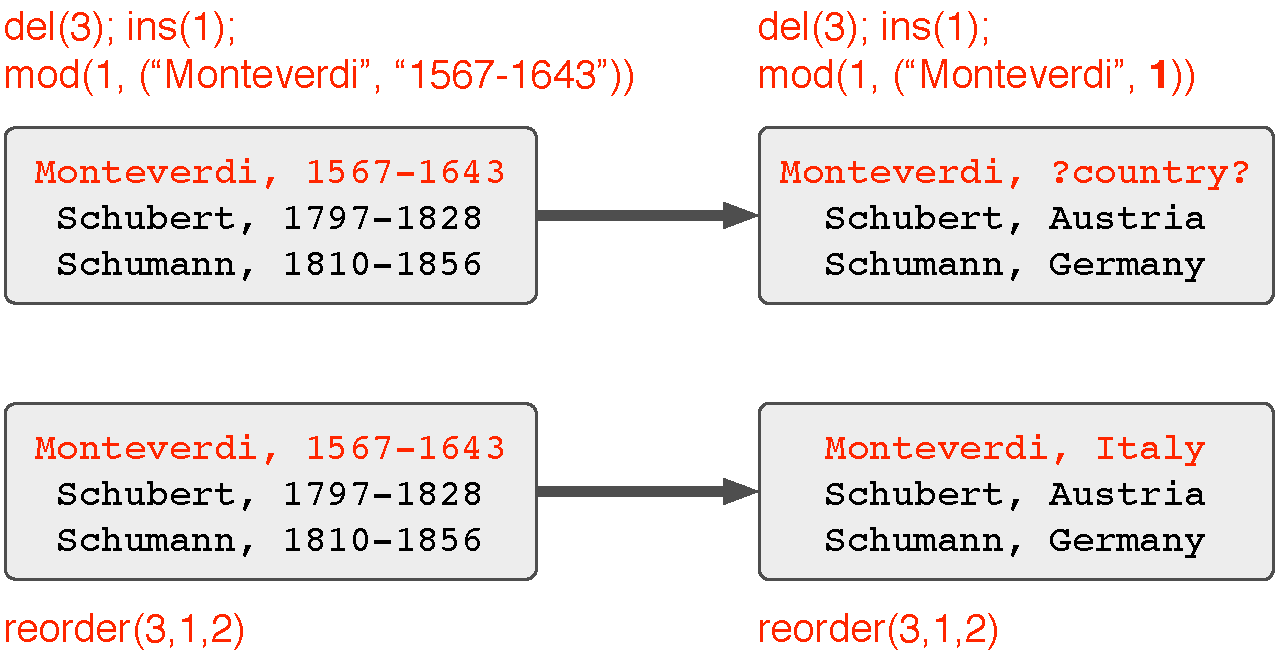
\includegraphics[width=75mm]{images/ex1-5.pdf} \\
        (f) two different edits with the same effect on the left
    \end{center}
    \caption{The desired behavior of a simple lens.}
    \label{fig:example-simple}
\end{figure}

\section{Symmetric lenses}
\label{sec:symmetric_lenses}
Lenses can be generalized from the asymmetric
presentation above---where one of the structures is always a ``view'' of the
other---to a
fully {\em symmetric} version where each of the two structures may
contain information that is not present in the other.
Although symmetric variants of lenses have been
studied~\cite{Meertens98,stevens2008tat,DBLP:conf/models/Diskin08}, they
all lack a notion of sequential composition of lenses, a significant
technical and practical limitation.
%
The extra structure needed to support composition is
nontrivial; in particular, constructions involving
symmetric lenses need to be proved correct modulo a notion of {\em behavioral
  equivalence}.
%
However, once that structure is in place, we find that there is a rich
\emph{algebra} on the space of lenses, which can be used as the theoretical
basis for a language of symmetric lenses.

The key step toward symmetric lenses is the notion
of {\em complements}.  The idea dates back to a famous paper in the
database literature on the view update
problem~\cite{DBLP:journals/tods/BancilhonS81} and was adapted to
lenses in~\cite{Matching10} (and, for a slightly different
definition,~\cite{matsuda2007btb}), and it is quite simple.  If we think of
the
\GET{} component of a lens as a sort of projection function, then we can find
another projection from $X$ into some set $C$ that
keeps all the information discarded by \GET{}.  Equivalently, we can think
of \GET{} as returning two results---an element of $Y$ and an element of
$C$---that together contain all the information needed to reconstitute the
original element of $X$.  Now the \PUT{} function doesn't need a whole $x\in
X$ to recombine with some updated $y\in Y$; it can
just take the complement $c\in C$ generated from $x$ by the \GET, since this
will
contain all the information that is missing from $y$.  Moreover, instead of
a separate
$\CREATE$ function, we can simply pick a distinguished element
$\missing\in C$ and define $\CREATE(y)$ as $\PUT(y,\missing)$.

So far, this perspective has retained the assumption that elements of $X$
have richer structure than elements of $Y$; hence, the complement need only
store the extra rich parts of $X$. For symmetry, we will lose this
assumption, and allow the complement set $C$ to contain information about
both $X$ elements and $Y$ elements. As a result, \emph{both} the \GET{} and
\PUT{} functions may need to inspect and update the complement. It will be
the responsibility of those functions to decompose the complement into the
``private information from $X$'' and the ``private information from $Y$'';
then we expect that \GET{} will read the part about $Y$ and write the part
about $X$ and \PUT{} will read the part about $X$ and write the part about
$Y$. Thus, our new types for \GET{} and \PUT{} are
\begin{align*}
    \aget &\in X \times C \arrow Y \times C \\
    \aput &\in Y \times C \arrow X \times C
\end{align*}
Note that the type is just ``lens from $X$ to $Y$'': the set
$C$ is an internal component, not part of the externally visible type.
In symbols, $ \mathit{Lens}(X,Y) =
\exists C.\; \{ \mathord{\missing}:\, C,\; \GET:\,X \times C \arrow Y
\times C,\; \PUT:\,Y \times C \arrow X \times C \}$.

Now that everything is symmetric, the \GET{} / \PUT{} distinction is not
helpful, so we rename the functions to \PUTR{} and \PUTL.  This brings us to
our core definition.

\iftikz
\iffull
\begin{figure*}[t!] \centering
\vspace*{-4ex}
\hspace*{-1em}
\begin{tabular}{@{}cc}
  \ifpdf\tikz\pdf{symmetric-minus};\vspace*{-1ex}
  \else \tikz\pdf{symmetric-minus}node[below=8.2ex]{};
  \fi
 &
  \tikz\pdf{symmetric};
  \ifpdf\vspace*{-2ex}\fi
 \\
(a) Initial replicas & (b) Initial complement
\vspace*{4ex} \\
  \ifpdf\tikz\pdf{symmetric-edit};\vspace*{-.7ex}
  \else \tikz\pdf{symmetric-edit}node[below=10ex]{};
  \fi
&
  \tikz\pdf{symmetric-propagatex};
\\
(c) One replica edited & (d) Propagating the edit
\vspace*{3ex}
\\
  \ifpdf\vspace*{3ex}\tikz\pdf{symmetric-edit2};\vspace*{-8ex}
  \else \tikz\pdf{symmetric-edit2}node[below=12.9ex]{};
  \fi
&
  \ifpdf\tikz\pdf{symmetric-propagate2};\vspace*{-1ex}
  \else \tikz\pdf{symmetric-propagate2}node[below=12.9ex]{};
  \fi
\\
(e) Second replica is edited & (f) This change is propagated
\vspace*{1.5ex}
\\
\end{tabular}
\caption{Behavior of a symmetric lens}\vspace*{2ex}
\label{fig:symm}
\end{figure*}
\else
\begin{figure*}[t!] \centering
\vspace*{-4ex}
\hspace*{-1em}
\begin{tabular}{@{}ccc}
  \ifpdf\tikz\pdf{symmetric-minus};\vspace*{-1ex}
  \else \tikz\pdf{symmetric-minus}node[below=8.2ex]{};
  \fi
 &
  \tikz\pdf{symmetric};
  \ifpdf\vspace*{-1ex}\fi
&
  \ifpdf\tikz\pdf{symmetric-edit};\vspace*{-3ex}
  \else \tikz\pdf{symmetric-edit}node[below=10ex]{};
  \fi
 \\
(a) Initial replicas & (b) Initial complement & (c) One replica edited
\vspace*{2ex} \\
  \tikz\pdf{symmetric-propagatex};
&
  \ifpdf\vspace*{3ex}\tikz\pdf{symmetric-edit2};\vspace*{-4ex}
  \else \tikz\pdf{symmetric-edit2}node[below=12.9ex]{};
  \fi
&
  \ifpdf\tikz\pdf{symmetric-propagate2};\vspace*{-1ex}
  \else \tikz\pdf{symmetric-propagate2}node[below=12.9ex]{};
  \fi
\\
(d) Propagating the edit & (e) Second replica is edited & (f) This change is propagated
\vspace*{1ex}
\\
\end{tabular}
\caption{Behavior of a symmetric lens}
\label{fig:symm}
\end{figure*}
\fi
\fi

\begin{definition}[Symmetric lens]
A lens $\ell$ from $X$ to
$Y$ (written $\ell \in X \lens Y$) has three parts:
a set of complements $C$, a distinguished element $\missing \in
C$, and two functions
\begin{eqnarray*}
    \putr &\in& X \times C \to Y \times C\\
    \putl &\in& Y \times C \to X \times C
\end{eqnarray*}
satisfying the following round-tripping laws:
\infrule[PutRL]{\putr(x,c) = (y,c')}{\putl(y,c') = (x,c')}
\infrule[PutLR]{\putl(y,c) = (x,c')}{\putr(x,c') = (y,c')}
When several lenses are under discussion, we use record notation to identify
their parts, writing $\ell.C$ for the complement set of $\ell$, etc.
\end{definition}

\iftext The force of the \rn{PutRL} and \rn{PutLR} laws is to establish some
``consistent'' or ``steady-state'' triples $(x,y,c)$, for which \PUT{}s of $x$
from the left or $y$ from the right will have no effect---that is, will not
change the complement. The conclusion of each rule has the same variable
$c'$ on both sides of the equation to reflect this.  We will use the
equation $\putr(x,c) = (y,c)$ to characterize the steady states.  In
general, a \PUT{} of a new $x'$ from the left entails finding a $y'$ and a
$c'$ that restore consistency.  Additionally, we often wish this
process to involve the
complement $c$ from the previous steady state; as a result, it can be
delicate to choose a good value of $\missing$. This value can often be
chosen compositionally; each of our primitive lenses and lens combinators
specify one good choice for $\missing$.

\iflater\finish{There's a good technical discussion of the options for
  dealing with creation in symmetric.v --- might be worth including it
  here.}\fi \fi

\iffull\else One can imagine other laws.  In particular, the long version of
the paper considers symmetric forms of the asymmetric ``\rn{PutPut}'' laws,
which specify that two \PUT{} operations in a row should have the same
effect as the second one alone.  As with asymmetric lenses, these
laws appear too strong to be desirable in practice.  \fi

%% %
%% We say that lenses $l$ and $l'$ are {\em equivalent} if there exists a
%% relation $\mathord{\equivl} \subseteq C \times \C{l'}$ such that:
%% \infax[MissingC]{l.\missing \equivl l'.\missing}
%% \infrule[PutrC]{
%%   c \equivl c'
%%   \andalso
%%   l.\PUTR (a, c) = (b,c_1)
%%   \andalso
%%   l'.\PUTR (a, c') = (b,c_1')
%% }{
%%   b = b' \ \wedge\   c_1 \equivl c_1'
%% }
%% \infrule[PutlC]{
%%   c \equivl c'
%%   \andalso
%%   l.\PUTL (b, c) = (a,c_1)
%%   \andalso
%%   l'.\PUTL (b, c') = (a,c_1')
%% }{
%%   a = a' \ \wedge\   c_1 \equivl c_1'
%% }

%% With these definitions in place, we can develop some basic
%% structure.  For every set $A$, we can define is an identity lens $\mathit{id}$
%% (with a trivial complement) from $A$ to itself.  If we have a lens $l$
%% from $A$ to $B$ and a lens $l'$ from $B$ to $X$, we can compose them to form
%% a lens $(l;l')$ from $A$ to $X$, using $l.C \times l'.C$ as the complement.
%% %
%% We can also show that, up to equivalence, composition is associative and
%% \emph{id} is its unit---i.e., symmetric lenses form a category.

%% \iffull \else \iftext \finish{Briefly mention the PutPut laws and the fact
%%   that, as usual, they are too strong.} \fi \fi
%% \iffull

\paragraph*{Examples} Figure~\ref{fig:symm} shows how this model might be
instantiated to synchronize the repositories discussed earlier in
Section~\ref{sec:asymm-limitations}.
%
The complement (b) contains all the information that is discarded by both
$\PUT$s---all the dates from the left-hand structure and all the countries
from the right-hand structure.  (It can be viewed as a pair of lists of
strings, or equivalently as a list of pairs of strings; the way we build
list lenses later actually corresponds to the latter.)  If we add a
new record to the left hand structure (c) and use the $\PUTR$ operation to
propagate it through the lens (d), we copy the shared information (the new
name) directly from left to right, store the private information (the new
dates) in the complement, and use a default string to fill in both the
private information on the right and the corresponding right-hand part of
the complement.  If we now update the right-hand structure to fill in the
missing information and correct a typo in one of the other names
(e), then a $\PUTL$ operation will propagate the edited country to the
complement, propagate the edited name to the other structure, and use the
complement to restore the dates for all three composers.

Viewed more abstractly, the
connection between the information about a single composer in the two tables
is a lens from $X \times Y$ to $Y \times Z$, with complement $X
\times Z$---let's call this lens $e$.  Its \PUTR{} component is given $(x,y)$ as
input and has $(x',z)$ in its complement; it constructs a new complement by
replacing $x'$ by $x$ to form $(x,z)$, and it constructs its output by
pairing the $y$ from its input and the $z$ from its complement to form
$(y,z)$. The \PUTL{} component does the opposite, replacing the $z$ part of
the complement and retrieving the $x$ part.  Then the
top-level lens in Figure~\ref{fig:symm}---let's call it
$e\LIST$---abstractly has type $(X \times Y)\LIST \lens (Y \times Z)\LIST$
and can be thought of as the ``lifting'' of $e$ from elements
to lists.

There are several plausible implementations of
$e\LIST$, with slightly different behaviors when list elements are
added and removed---i.e., when the input and complement arguments to \PUTR{}
or \PUTL{} are lists
of different lengths.  One possibility is to take $e\LIST.C = (e.C)\LIST$
and maintain the invariant that the complement list in the output is the same length as
the input list. When the lists in the input have different lengths, we can
restore the
invariant by either truncating the complement list or padding it with
$e.\missing$.
% \iffull
For example, taking $X = \{a,b,c,\ldots\}$, $Y = \{1,2,3,\ldots\}$, $Z =
\{A,B,C,\ldots\}$, and $e.\missing = (m,M)$, and writing
$\left<a,b,c\right>$ for the sequence with the three elements $a$, $b$, and
$c$, we could have:
\[
\begin{array}{ll}
& \PUTR (\left<(a,1)\right>,\;
         \left<(p,P),(q,Q)\right>)
\\
= &\PUTR (\left<(a,1)\right>,\;
         \left<(p,P)\right>)\mbox{\hspace{7.7em}(truncating)}
\\
= & ( \left<(1,P)\right>,\; \left<(a,P)\right>)
\\ [1.5ex]
& \PUTR (\left<(a,1),(b,2)\right>,\;
         \left<(a,P)\right>)
\\
= &\PUTR (\left<(a,1),(b,2)\right>,\;
         \left<(a,P),(m,M)\right>)\mbox{\qquad(padding)}
\\
= & (\left<(1,P),(2,M)\right>,\;
         \left<(a,P),(b,M)\right>)
\end{array}
\]
% \fi
Notice that, after the first \PUTR{}, the information in the second
element of the complement list $(q,Q)$ is lost.
The second \PUTR{} creates a brand new second element for the list, so the value $Q$ is
gone forever; what's left is the default value $M$.

\iftikz
\begin{figure*}[t!] \centering
\vspace*{-4ex}
\begin{tabular}{@{}ccc}
  \tikz\pdf{sums1};
  &
  \tikz\pdf{sums2};
  \ifpdf\else\vspace*{2ex}\fi
  \\
  (a) Initial replicas & (b) Alphabetizing the right
  \vspace*{2ex} \\
  \tikz\pdf{sums3};
  &
  \tikz\pdf{sums4};
  \ifpdf\else\vspace*{2ex}\fi
  \\
  (c) Inserting Chopin on the left & (d) Deleting Beethoven from the left
\end{tabular}
\caption{Synchronizing lists of sums}
\label{fig:sums}
\end{figure*}
\fi
Figure~\ref{fig:sums} illustrates another use of symmetric lenses. The
structures in this example are lists of categorized data; each name on the
left is either a composer (tagged {\tt inl}) or an author (tagged
{\tt inr}), and each name
on the right is either a composer or an actor.  The
lens under consideration will synchronize just the composers between the two
lists, leaving the authors untouched on the left and the actors untouched on
the right. The synchronized state (a) shows a complement with two lists,
each with holes for the composers.  If we re-order the
right-hand structure (b), the change in order will be
reflected on the left by swapping the two composers. Adding another composer
on the left
(c) involves adding a new hole to each complement; on the left, the location
of the hole is determined by the new list, and on the right it simply shows
up at the end. Similarly, if we remove a composer (d), the
final hole on the other side disappears.

Abstractly, to achieve this behavior we need to define a lens $\comp$
between $(X+Y)\LIST$ and
$(X+Z)\LIST$.  To do this, it is convenient to first define a lens that
connects $(X+Y)\LIST$ and $X\LIST \times Y\LIST$; call this lens $\partition$.
The complement of the $\partition$ is a list of booleans telling whether the
corresponding element of the left list is an $X$ or a $Y$. The $\putr$
function is fairly simple: we separate the $(X+Y)$ list into $X$ and $Y$
lists by checking the tag of each element, and set the complement to exactly
match the tags. For example:
\begin{align*}
\putr(\left<\mlinl a,\mlinl b,\mlinr 1\right>,c) &=
    ((\left<a,b\right>,\left<1\right>),\left<\false,\false,\true\right>) \\
\putr(\left<\mlinl a,\mlinr 1,\mlinl b\right>,c) &=
    ((\left<a,b\right>,\left<1\right>),\left<\false,\true,\false\right>)
\end{align*}
These examples demonstrate that $\putr$ ignores the complement entirely,
fabricating a completely new one from its input. The $\putl$ function, on
the other hand, relies entirely on the complement for its ordering
information. When there are extra entries (not accounted for by the
complement), it adds them at the
end. Consider taking the output of the second $\putr$ above and
adding $c$ to the $X$ list and $2$ to the $Y$ list:
\\[1.5ex]
\noindent\begin{tabular}{l}
$\putl((\left<a,b,c\right>,\left<1,2\right>),\left<\false,\true,\false\right>) =$ \\
\qquad$(\left<\mlinl a,\mlinr 1,\mlinl b,\mlinl c,\mlinr 2\right>,$ \\
\qquad$\left<\false,\true,\false,\false,\true\right>)$
\end{tabular}
\\[1.5ex]
\noindent The $\putl$ fills in as much of the beginning of the list as it
can, using the complement to indicate whether to draw elements from $X\LIST$
or from $Y\LIST$.  (How the remaining $X$ and $Y$ elements are interleaved
is a free choice, not specified by the lens laws, since this case only
arises when we are {\em not} in a round-tripping situation. The strategy
shown here, where all new $X$ entries precede all new $Y$ entries, is just
one possibility.)

Given $\partition$, we can obtain $\comp$ by composing three lenses in
sequence: from $(X+Y)\LIST$ we get to $X\LIST \times Y\LIST$ using
$\partition$, then to $X\LIST \times Z\LIST$ using a variant of the lens $e$
discussed above, and finally to $(X+Z)\LIST$ using a ``backwards''
$\partition$.

% TODO: things we know that aren't discussed here:
% - all the lens operations needed to implement the transformations we
%   discussed here, plus some for containers
% - recursion (right?)
% - machinery needed to show these operations are ``well-behaved'' (in
%   particular, have categorical descriptions)
% - exploration of different choices for several operators that are still
%   ``well-behaved'', and their tradeoffs

\iffull

\section{Edit lenses}
\label{sec:edit_lenses}
The two frameworks discussed, asymmetric state-based lenses and symmetric
state-based lenses, are both somewhat ``extensional''. That is: the
\PUT{} functions have access only to extensional information about the
states of the repository before and after any user changes. As shown in (f)
of Figure~\ref{fig:example-simple}, this information is not always enough to
determine a best modification to the unchanged repository to restore
synchrony: one wants ``intentional'' information about how a change was made
in addition to the effect that change had. Additionally, the description of
what has changed since the last synchronization point can often be
represented much more compactly than the new value of the repository. The
goal of edit lenses is to address these two concerns.

We do not address the question of where these edits come from or who
decides, in cases like part (f), which of several possible edits is
intended.  As argued in~\cite{Matching10}, answers to these questions will
tend to be intertwined with the specifics of particular editing and/or
diffing tools and will tend to be messy, heuristic, and
domain-specific---unpromising material for a foundational theory.  Rather,
our aim is to construct a theory that shows how edits, however
generated, can be translated between replicas of different shapes.

Below, we discuss how to build an edit lens synchronizing the data
structures in the introductory example in Figure~\ref{fig:example-simple},
paralleling the discussion of symmetric lenses. The primary difference is
that each lens must also be associated with the set of edits that it knows
how to translate. In the following, we will discuss how to build this
association compositionally; the role that complements play in edit lenses;
and the formal definition of edit lenses.

\subsection{Building edit languages}
As with symmetric lenses, we will build our edit lens between $(X \times
Y)^*$ and $(X \times Z)^*$ compositionally---that is, the whole lens
should have the form $\ell^*$, where $*$ is a ``list mapping'' lens
combinator and $\ell$ itself is a product $\ell_1 \times
\ell_2$ of a lens $\ell_1 \in X \to X$ that translates composer edits
verbatim, while $\ell_2 \in Y \to Z$ is a ``disconnect'' lens that maps every edit on
either side to a trivial identity edit on the other side.

In analogous fashion, the edit languages for the top-level structures will
be constructed compositionally.  The set of edits for structures of the form
$(X \times Y)^*$, written $\partial ((X \times Y)^*)$, will be defined
together with the list constructor $*$.  Its elements will have the form
$\mlins{i}$ where $i$ is a position, $\mldel{i}$,
$\mlreorder{i_1,\ldots,i_n}$ where $i_1,\ldots,i_n$ is a permutation on
positions (compactly represented, e.g. as a branching program),
\iflater\discuss{people will be suspicious here---how do we know we
  can represent it compactly?}\fi and $\mlmod{p}{\dv}$, where $\dv \in
\partial (X\times Y)$ is an edit for $X \times Y$ structures.  Pair edits
$\dv \in \partial (X \times Y)$ have the form $\partial X \times
\partial Y$, where $\partial X$ is the set of edits to composers and
$\partial Y$ is the set of edits to dates.  Finally, both $\partial
X$ and $\partial Y$ are sets of primitive ``overwrite edits'' that completely
replace one string with another, together with an identity edit $\ONE$
that does nothing at all; so $\partial X$ can be just $\{\unit\} + X$ (with
$\ONE = \mlinl\unit$) and similarly for $Y$ and $Z$.

%% We write $\ONE$ instead of $\mlinl\ONE$ and {\sf
%%   ``x''} instead of $\mlinr x$ in contexts where it is clear that an edit of
%% this form is expected.

%% We can represent an edit to an element of $X \times Y$ as a pair of
%% edits to $X$ and $Y$; that is, $\partial(X \times Y) = \partial X \times
%% \partial Y$.  The application function $\odot_{X \times Y}$ simply applies
%% each of the component edits to the appropriate parts of the
%% product:
%% \iffull \[ \else $ \fi
%% (\dx,\dy) \odot_{X \times Y} (x, y) = (\dx \odot_X x, \dy \odot_Y y)
%% \iffull .\] \else $. \fi
%% We sometimes write $\mlonl\dx$ as an alias for $(\dx,\ONE)$ when we want to
%% emphasize that a particular edit affects only one part of a tuple, and
%% similarly for $\mlonr\dy$.

Our lens $\ell^*$ will consist of two components---one for transporting edits
from the left side to the right, written $(\ell^*).\dputr \in \partial(X
\times Y)^* \to \partial(X \times Z)^*$,\footnote{The symbol $\dputr$ is
  pronounced ``put an edit through the lens from left to right,'' or just
  ``put right.''  It is the {\edit}-analog of the $\putr$ function.} and another for transporting
edits from right to left, written $(\ell^*).\dputl \in \partial(X \times
Z)^* \to \partial(X \times Y)^*$.
%

% TODO: part of the point of this is that all that can be done without
% complements, and this point needs to be made somehow for the next section
% to make sense

%% The next step is to lift this translation to lists.  There are two kinds of
%% edits to lists in the example\finish{why is it this way?}:
%% \emph{rearrangements}, which modify the
%% structure of the list via insertions of dummy elements, deletions,
%% reorderings (but which do not modify the elements themselves), and
%% \emph{modifications} of the values in the list using the underlying element
%% edits (which do not affect the list structure or order).  We already know
%% how to translate modifications, and rearrangements are easy because the list
%% structure is the same on both sides.  Putting these observations together
%% gives us a translation function $\ell^*.\dputr \in \partial((X\times Y)^*)
%% \to \partial((X \times Z)^*)$ for list edits (the $\dputl$ function is
%% similar):
%% \iffull
%%   \begin{align*}
%%     \ell^*.\dputr(\mlins i) &= \mlins i \\
%%     \ell^*.\dputr(\mldel i) &= \mldel i \\
%%     \ell^*.\dputr(\mlreorder{i_0,\ldots,i_n}) &= \mlreorder{i_0,\ldots,i_n} \\
%%     \ell^*.\dputr(\mlmod ie) &= \mlmod i{\ell.\dputr(e)}
%%   \end{align*}
%% \else
%% \[
%% \begin{array}{lcl}
%%     \ell^*.\dputr(\di) &=& \di \\&& \mbox{if $\di$ is an $\mlins$,
%%     $\mldel$, or $\mlreorder$}\\
%%     \ell^*.\dputr(\mlmod ie) &=& \mlmod i{\ell.\dputr(e)}
%% \end{array}
%% \]
%% \fi
%% \iflater
%% \bcp{Not exactly sure what we want to say about this---cutting from the
%%   short version.}
%% The reader may wonder why we break list insertions into
%% two stages---first inserting a dummy element and then modifying this dummy
%% element with desired data. The ease of writing the above function is
%% the answer: since the former stage does not mention elements of the list at
%% all, we need not do any translation, and since the latter stage is
%% simply an edit script, we may dispatch to the underlying lens.
%% \fi
%% %% Additionally,
%% %% the breakdown lets us preserve a nice factorization property that we discuss
%% %% in the next section.\bcp{where? refer to it by number?}

\subsection{Complements}
\begin{figure}
    \begin{tabular}{c}
        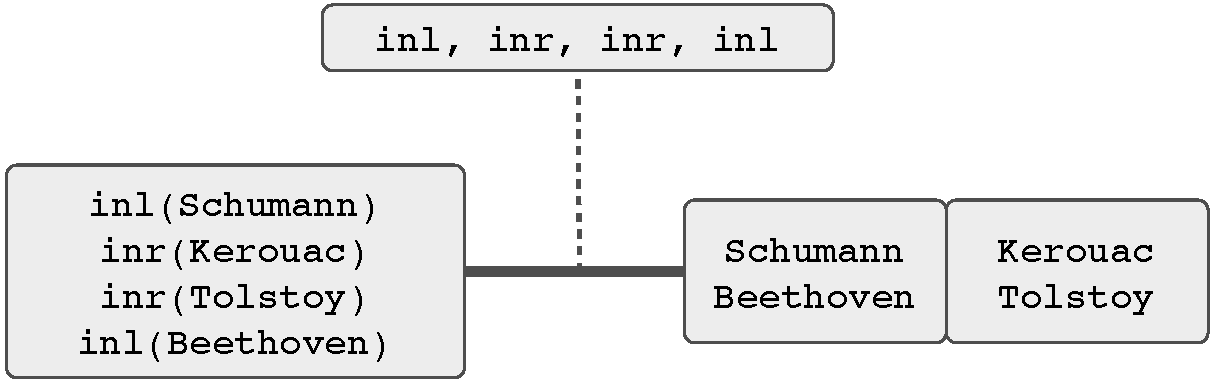
\includegraphics[width=75mm]{images/ex2-0.pdf} \\[.9ex]
        \parbox \linewidth{(a) the initial replicas: a tagged list of composers and authors on
        the left; a pair of lists on the right; a complement storing just
        the tags}
        \\[3ex]
        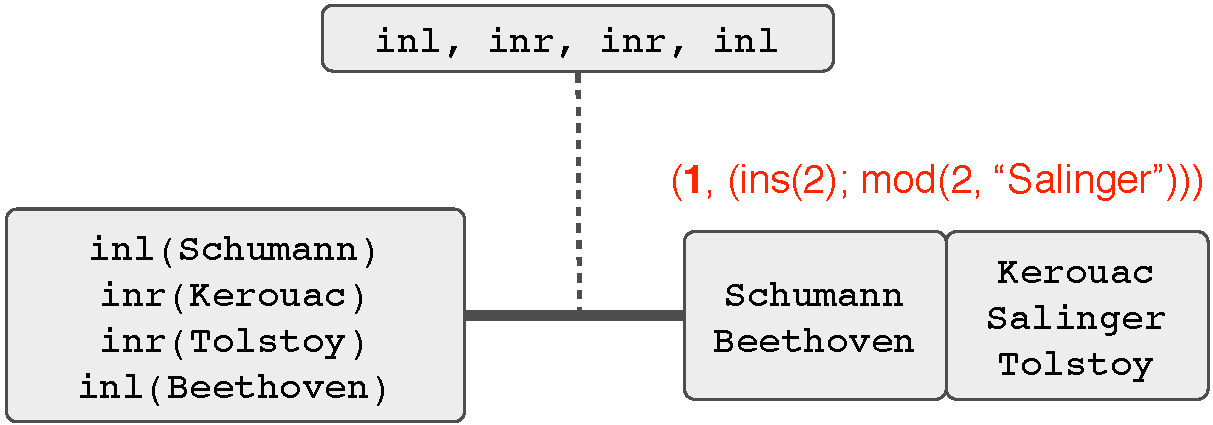
\includegraphics[width=75mm]{images/ex2-1.pdf} \\
        \parbox \linewidth{\begin{center}(b) an element is added to one of
            the partitions\end{center}} \\[2ex]
        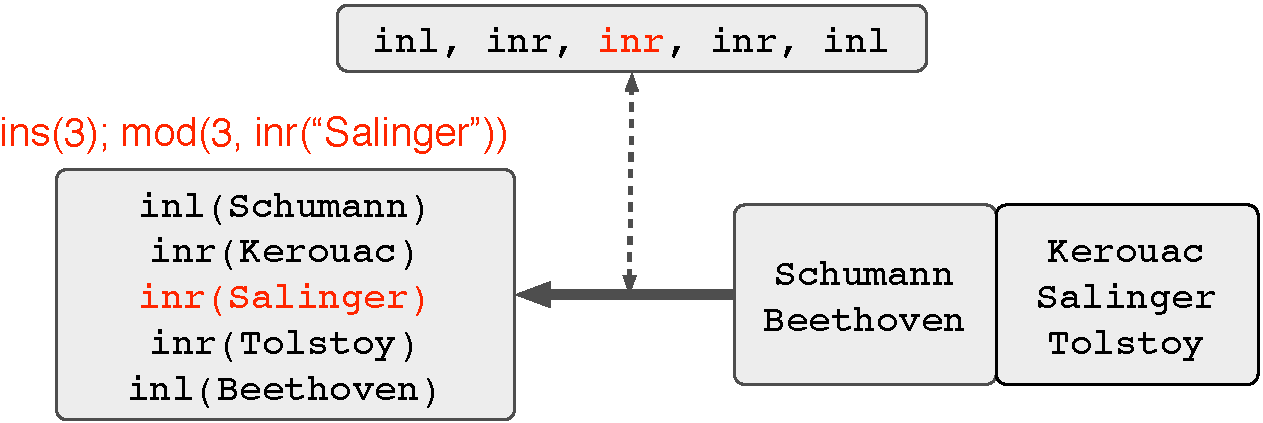
\includegraphics[width=75mm]{images/ex2-2.pdf} \\
        \parbox \linewidth{\begin{center}(c) the complement tells how to translate the
            index\end{center}} \\[.7ex]
    \end{tabular}
    \caption{A lens with complement.}
    \label{fig:example-partition}
\end{figure}

We sometimes need lenses to have a little more structure than this simple
example suggests.
To see why, consider defining a {\em partitioning} lens $p$ between
the sets $\partial((X+Y)^*)$ and $\partial(X^* \times Y^*)$.
Figure~\ref{fig:example-partition} demonstrates the behavior of this lens.
%
In part (a), we show the original replicas: on the left, a single list that
intermingles authors and composers (with {\sf inl/inr} tags showing which is
which), and on the right a pair of homogeneous (untagged) lists, one for
authors and one for composers. Now consider an edit, as in (b), that inserts
a new element somewhere in the author list on the right. It is clear that we
should transport this into an insertion on the left replica, but where, exactly,
should we insert it?  If the $\dputl$ function is given just an
insertion edit for the homogeneous author list and nothing else, there is no
way it can translate this edit into a sensible position in the combined list
on the left, since it doesn't know how the lists of authors and composers
are interleaved on the left.

\iflater\bcp{People were not clear on why the complement was needed.  Also, in this
  example, even with the complement, there is still some arbitrary choice in
  where an inserted element on the right appears in the list on the left.}\fi

The solution is to store a complement off to the
side, recording the \emph{tags} ($\ml{inl}$ or $\ml{inr}$) from the
original, intermingled list, and pass this list as an extra argument to
translation.  We then enrich the types of the edit translation functions to
accept a complement and return a new complement, so that
%
\iffull \[ \else $ \fi
p.\dputr \in \partial((X+Y)^*) \times C \to \partial(X^* \times Y^*)
\times C
\iffull \] \else $ \fi
and
\iffull \[ \else $ \fi
p.\dputl \in \partial(X^* \times Y^*) \times C \to \partial((X+Y)^*)
\times C
\iffull .\] \else $. \fi
Part (c)
demonstrates the use (and update) of the complement when translating the
insertion.

Note that the complement stores just the {\sf inl/inr} tags, not the actual
names of the authors and composers in the left-hand list.  \iflater\finish{This next
statement made people suspicious---we need to go into more detail.}\fi In general, the
information stored in $C$ will be much smaller than the
information in the replicas; indeed, our earlier example illustrates the
common
case in which $C$ is the trivial single-element set $\Unit$.  The
translation functions manipulate just the complements and the edits, which
are also small compared to the size of the replicas.

%% \finish{Someplace, we need to talk about what happens to edits that don't
%%   make sense on the current state.  There are three possibilities, with a
%%   tradeoff between size of representations and ``accuracy'' of edits:
%%   \begin{itemize}
%%   \item Embed a description of the exact state in the edit and say that the
%%   edit only applies to this state.  This is what Diskin, etc., do.  But it
%%   means that edits are very large.
%%   \item Allow any edit to apply to any state.  Then there are two
%%   sub-possibilities:
%%   \begin{itemize}
%%   \item keep it total but make it behave like the identity (or some other
%%   arbitrary choice) anywhere it doesn't ``make sense''
%%   \item make it partial
%%   \end{itemize}
%%   \end{itemize}
%% }
%% \finish{
%% Old text: Other authors model {\edit}s in other ways; for example, Stevens
%% \finish{citation} chooses functions whose domain and range are equal.
%% Functions are a nice model in some circumstances, but are difficult to
%% inspect: the only operation that can be performed is to apply them to some
%% concrete argument.  Monoids subsume these functions, and some instantiations
%% offer more reflective representations of edits.}

\subsection{Formal definition}
\label{sec:semantics}

A key design decision in our formulation of edit lenses is to separate the
{\em description} of edits from the {\em action} of applying an edit to a
state.  This separation is captured by the standard mathematical notions of
{\em monoid} and {\em monoid action}.

\begin{definition}
%% \bcp{why do we say a triple here and in
%%     3.2.3, but other places just name the components (e.g., defn of
%%     category)?}
A \emph{monoid} is a triple $\left<M,\cdot_M,\ONE_M\right>$ of a set
$M$, an associative binary operation $\cdot_M \in M \times M
\to M$, and a unit element $\ONE_M \in M$ --- that is, with $\cdot_M$ and $\ONE_M$ such that
\iffull
\begin{eqnarray*}
x\cdot_M(y\cdot_M z) = (x\cdot_M y) \cdot_M z\\
\ONE_M\cdot_M x = x = x \cdot_M \ONE_M .
\end{eqnarray*}
\else
$x\cdot_M(y\cdot_M z) = (x\cdot_M y) \cdot_M z $ and
$\ONE_M\cdot_M x = x = x \cdot_M \ONE_M$.
\fi
\end{definition}
When no confusion results, we use $M$ to denote both the set and the
monoid, drop subscripts from $\cdot$ and $\ONE$, and write $mn$ for
$m \cdot n$.
%% In more standard terminology, a ``monoid'' in our sense would
%% be called a \emph{partial monoid}\iflater~\cite{partialmonoids}\fi, but
%% since we always work with partial monoids we find it convenient to drop the
%% qualifier.

The unit element represents a ``change nothing'' edit.  Multiplication of
edits corresponds to packaging up multiple edits into a single one
representing their combined effects\iffull{} (this might be useful, for example, for
offline editing)\fi.

Modeling edits as monoid elements gives us great flexibility in
concrete representations.
%
The simplest edit language is a {free monoid} whose elements are just words
over some set of primitive edits and whose multiplication is
concatenation.
%
However, it may be useful to put
more structure on edits, either (a) to allow
more compact representations or (b) to capture the intuition that edits to
different parts of a structure do not interfere with each other and can thus
be applied in any order.
%
The monoid framework can also accommodate more abstract notions of edit.  For
example, the set of all total functions from a set $X$ to itself forms a
monoid, where the multiplication operation is function composition.  This is
essentially the form of edits considered by
Stevens~\cite{stevens2008tat}\iflater\finish{Not just Stevens---we should
  find a few more citations for this idea.}\fi.  \iflater\bcp{Same question for this one.  At a minimum, we should say that we are not dealing with these examples in detail in the rest of the paper.}\fi
%
We mostly focus on the simple case where edit languages are free monoids.
Laws can be added to the product and sum lens constructions, and possibly
for lists and general containers as well.

\begin{definition}
    Given a  monoid $M$ and a set $X$, a \emph{monoid action} on $M$ and $X$
    is a partial function $\odot \in M \times X \partialto X$ satisfying two laws:
\iffull
    \infax{\ONE \odot x = x}
    \infax{(m \cdot n) \odot x = m \odot (n \odot x)}
\else
$\ONE \odot x = x$ and $(m \cdot n) \odot x = m \odot (n \odot x)$.
\fi
\end{definition}
%
As with monoid multiplication, we often elide the monoid action symbol,
writing $mx$ for $m \odot x$.  In standard mathematical terminology, a
monoid action in our sense might instead be called a ``partial monoid
action,'' but since we always work with partial actions we find it
convenient to drop the qualifier.

A bit of discussion of partiality is in order.
Multiplication of edits is a total operation: given two descriptions of
edits, we can always find a description of the composite actions of doing
both in sequence.  On the other hand, {\em applying} an edit to a particular
state may sometimes fail.
%
This means we need to work with expressions and equations involving
partial operations. As usual, any term that contains an undefined
application of an operation to operands is undefined---there is no way of
``catching'' undefinedness. An equation between possibly undefined terms
(e.g., as in the definition above)
means that if either side is defined then so is the other, and their values
are equal (Kleene equality).

Why deal with failure explicitly, rather than keeping edit application total
and simply defining our monoid actions so that applying an edit in a state
where it is not appropriate yields the same state again (or perhaps some
other state)?  One reason is that it seems natural to directly address the
fact that some edits are not applicable in some states, and to have a
canonical outcome in all such cases.  A more technical reason is that, when
we work with monoids with nontrivial equations, making inapplicable edits
behave like the identity is actually
wrong.%
%
\footnote{Here is a slightly contrived example.  Suppose that the set of
  states is natural numbers and that edits have the form $(x\mapsto y)$,
  where the intended interpretation is that, if the current state is $x$,
  then the edit yields state $y$.  It is reasonable to impose the equation
  $(y\mapsto z)\cdot(x\mapsto y) = (x\mapsto z)$, allowing us to represent
  sequences of edits in a compact form.  But now consider what happens when
  we apply the edit $(5\mapsto 7)\cdot(3\mapsto 5)$ to the state $5$.  The
  second monoid action law demands that $((5\mapsto 7)\cdot(3\mapsto 5))
  \odot 5 = (5\mapsto 7)\odot((3\mapsto 5) \odot 5)$, which, by the equation
  we imposed, is the same as $(3\mapsto 7) \odot 5 = (5\mapsto
  7)\odot((3\mapsto 5) \odot 5)$.  But the left-hand side is equal to $5$
  (since the edit $(3\mapsto 7)$ does not apply to the state $5$), while the
  right-hand side is equal to $7$ (since the first edit, $(3\mapsto 5)$, is
  inapplicable to the state $5$, so it behaves like the identity and returns
  $5$ from which $(5\mapsto 7)$ takes us to $7$), so the action law is
  violated.}

However, although the framework allows for the possibility of edits failing,
we still want to know that the edits produced by our lenses will never
actually fail when applied to replica states arising in practice.  This
requirement, corresponding to the {\em totality} property of previous
presentations of lenses~\cite{Focal2005}, is formalized and proven.
In general, we adopt the design principle that partiality
should be kept to a minimum; this simplifies the definitions.

%% Notice that the second law implies that if $m\odot(n\odot x)$ is
%% defined then $m\cdot n$ must be defined and conversely, if $n\odot x$
%% is undefined then $(m\cdot n)\odot x$ must also be undefined for all
%% $m$ even if $m\cdot n$ is defined.

\iflater
\finish{A monoid action is a monoid homomorphism from $M$ to $X \to X$. Can
tie this back to the Stevens work, too, maybe?}
\fi

It is convenient to bundle a particular choice of monoid and monoid
action, plus an initial element, into a single structure:

\begin{definition}
    A \emph{module} is a tuple $\left<X,\, \init_X,\, \partial
    X,\,\odot_X\right>$ comprising a set $X$, an element $\init_X\in X$, a monoid
    $\partial X$, and a monoid action $\odot_X$ of $\partial X$ on $X$.
\end{definition}
If $X$ is a module, we refer to its first component by either
$|X|$ or just $X$, and to its last component by $\odot$ or simple
juxtaposition.

We will use modules to represent the structures connected by lenses.  Before
coming to the definition of lenses, however, we need one last ingredient:
the notion of a {\em stateful homomorphism} between monoids.  As we saw in
the examples, there are situations where the information in an
edit may be insufficient to determine how it should be translated---we may
need to know something more about how the two structures correspond. The
exact nature of the extra information needed varies according to the lens.
%
To give lenses a place to store such auxiliary information, we
follow~\cite{HofmannPierceWagner10} and allow the edit-transforming
components of a lens (the $\dputr$ and $\dputl$ functions) to take a {\em
  complement} as an extra input and return an updated complement as an extra
output.
%
\iflater
\discuss{Not sure there's time to change it now, but I found while writing
  that explanation that the word ``complement'' was quite awkward---I kept
  wanting to say just ``state.''  Moreover, the term is technically a bit
  tenuous now, since what we store is not, in fact, anything like a
  complement in the old database sense.}  \soon{complement becomes correspondence}
\fi

\begin{definition}
Given monoids $M$ and $N$ and a {\em complement set} $C$, a \emph{stateful monoid
  homomorphism} from $M$ to $N$ over $C$ is a function $h \in M \times C \to
N \times C$ satisfying two laws:
%
\vspace*{-1ex}
\infrule{}{h(\ONE_M,c) = (\ONE_N,c)}
\infrule{
         h(m,c) = (n,c') \andalso h(m',c') = (n',c'')
}{
         h(m' \cdot_M m,c) = (n' \cdot_N n,c'')
}
%
These are basically just the standard monoid homomorphism laws, except that
$h$ is given access to some internal state $c \in C$ that it uses (and
updates) when mapping from $M$ to $N$; in the second law, we must thread the
state $c'$ produced by the first $h$ into the second use of $h$, and we
demand that both the result and the effect on the state should be the same
whether we send a composite element $m' \cdot m$ through $h$ all at once or
in two pieces.
\end{definition}

The intended usage of an edit lens is as follows. There are two users,
one holding an element of $X$ the other one an element of $Y$, both
referred to hereafter as {\em replicas}.  Initially, they hold $\init_X$ and
$\init_Y$, respectively, and the lens is initialized with complement
$\ell.\missing$. The users then perform actions and propagate them across
the lens. An action consists of producing an edit $\dx$ (or $\dy$), applying
it to one's current replica $x$ (resp.\ $y$), putting the edit through the lens
to obtain an edit $\dy$ (resp.\ $\dx$), and asking the user on the other
side to apply $\dy$ ($\dx$) to their replica.  In the process, the internal
state $c$ of the lens is updated to reflect the new correspondence between
the two replicas.
\iffull

\fi%
We further assume there is some {\em consistency} relation $K$ between $X$,
$Y$, and $C$, which describes the ``synchronized states'' of the replicas
and complement.  This gives us a natural way to state the totality
requirement discussed above: if we start in a consistent state, make a
successful edit (one that does not fail at the initiating side), and put it
through the lens, the resulting edit is guaranteed (a) to be applicable on
the receiving side and (b) to lead again to a consistent state.  We make no
guarantees about edits that fail at the initiating side: these should not be
put through the lens.

\begin{definition}
A \emph{symmetric edit lens} between modules $X$ and $Y$ consists of a
complement set $C$, a distinguished element $\missing\in C$,
two stateful monoid homomorphisms
\iffull
\[
\begin{array}{lcl}
\dputr &\in& \partial X \times C \to \partial Y \times C \\
\dputl &\in& \partial Y \times C \to \partial X \times C
\end{array}
\]
\else
$\dputr \in \partial X \times C \to \partial Y \times C$ and
$\dputl \in \partial Y \times C \to \partial X \times C$,
\fi
%
%% total functions
%% \[
%% \begin{array}{lcl}
%% \dputr &\in& \partial X \times C \to \partial Y \times C \\
%% \dputl &\in& \partial Y \times C \to \partial X \times C
%% \end{array}
%% \]
%% such that \infax{\dputr(\ONE,c)=(\ONE,c) \qquad \dputl(\ONE,c)=(\ONE,c)}
%% \infrule{ \dputr(\dx_2,c)=(\dy_2,c') \quad
%%   \dputr(\dx_1,c')=(\dy_1,c'') }{ \dputr(\dx_1\ \dx_2,c)=(\dy_1\
%%   \dy_2, c'') } \infrule{ \dputl(\dy_2,c)=(\dx_2,c') \quad
%%   \dputl(\dy_1,c')=(\dx_1,c'') }{ \dputl(\dy_1\ \dy_2,c)=(\dx_1\
%%   \dx_2, c'') }
and a ternary {\em consistency relation}
$K\subseteq |X|\times C\times |Y|$ such that
\begin{itemize}
\item $(\init_X,\missing,\init_Y)\in K$;
\item if $(x,c,y)\in K$ and $\dx\ x$ is defined and $\dputr(\dx,c)=(\dy,c')$, then $\dy\ y$ is also defined and $(\dx\ x,c',\dy\ y)\in K$;
\item if $(x,c,y)\in K$ and $\dy\ y$ is defined and $\dputl(\dy,c)=(\dx,c')$, then $\dx\ x$ is also defined and $(\dx\ x,c',\dy\ y)\in K$.%
%
\iffull
\footnote{One might consider a more general format with ``creation''
  operations $\creater\in X\rightarrow Y\times C$ and symmetrically
  $\createl$.  This format actually arises as a special case of the one
  above by choosing the edit monoids to include operations of the form
  $\text{set}(x)$ for $x\in X$, with action $\text{set}(x)\odot x'=x$. One
  can then define $\creater(x,c) = \dputr(\text{set}(x),c)$.}
\fi
%
\end{itemize}
% \discuss{BCP will add a note about binary consistency relations.  Dual role: Important sanity check on dputs, but also a part of the external specification of the lens.}
\end{definition}
